% !TEX root = ./report.tex
Bipartite graphs are used in multiple problem domains to represent the relationships between pairs of disparate data types.
Interpreting these relationships is often achieved by enumerating the maximal bicliques in a given bipartite graph, a computationally challenging task.
Zhang \emph{et al.} provide the most efficient currently known algorithm~\cite{Zhang2014} for carrying out this task.
In fact, they give two slightly different algorithms.
This report describes the implementation of these two algorithms for MPHYG002, coursework 1.

\section{Background}
Now let us look at the problem in detail.
A \emph{bipartite graph} is a graph whose vertices can be partitioned into a pair of non-empty, disjoint partitions such that no two vertices in the same partition are connected by an edge.
Let $G= (U\cup V, E)$ be a bipartite graph, with $U$ and $V$ denoting its two vertex set partitions, and $E$ denoting its edge set.
A bipartite graph $G$ can be described by its $\abs{U}\times \abs{V}$ \emph{biadjacency matrix}, $A_G$, with elements defined as follows
\begin{equation}\label{eq:biadjacency}
    [A_G]_{i,j} = \begin{cases}
    1, & \text{iff $(i,j)\in E$};\\
    0, & \text{otherwise};
\end{cases}
\qq{for all $i\in U,\ j \in V$}. 
\end{equation}
A \emph{biclique} $C = (U', V')$ is a subgraph of $G$ induced by a pair of disjoint subsets $U'\subseteq U$, $V' \subseteq V$, such that for all $u\in U'$, $v \in V'$, $(u,v)\in E$.
More informally, a biclique in $G$ is a fully connected subgraph of $G$.
A \emph{maximal biclique} $C = (U',V')$ in $G$ is a biclique for which there is no additional vertex in $V\cup U$ which you can add to $C$ and it still remain a biclique.

\begin{wrapfigure}{r}{0.5\textwidth}
    \centering
    \includegraphics[width=0.25\textwidth]{crown}
    \caption{
    A crown graph on ten vertices.
    There are $2^{5}-2 = 30$ maximal bicliques in this graph.
    For every subset of $U$ (apart from $\emptyset$ and $U$ itself), the induced subgraph is a unique maximal biclique. 
    }
    \label{fig:crown}
\end{wrapfigure}

\par
The problem we are interested in is the enumeration of all the maximal bicliques of a given bipartite graph $G$.
This problem is intrinsically computationally hard since in some cases, the number of maximal bicliques in a bipartite graph can be exponential in the number of vertices.
An example of such a graph is the \emph{crown graph}, an example of which is shown in Figure~\ref{fig:crown}.
For any crown graph on $2n$ vertices, there are $2^n - 2$ maximal bicliques.

\par
The algorithms by Zhang \emph{et al.} are called the (improved) Maximum Biclique Enumeration Algorithm, or iMBEA and MBEA respectively.
MBEA roughly works by recursively choosing subsets of one of the vertex partitions and checking if the induced subgraph is a biclique and if this biclique is maximal.
iMBEA is essentially the same as MBEA, but takes actions to prune the recursion tree of paths which won't lead to maximal bicliques and to decrease the lengths of paths which do.
The detailed algorithms can be seen in~\cite[Algorithm: MBEA]{Zhang2014}.

\section{Implementation}
The C++ program written for this work, implementing both MBEA and iMBEA is called \texttt{MBEA}.
It is a command line program which takes as input the location of a text file and a parameter to decide between MBEA and iMBEA.
The text file should contain the biadjacency matrix of a graph.
The program then prints a list of the maximal bicliques in the graph, according to the vertex labelling implicitly defined by the input biadjacency matrix, as well as the total number of maximal bicliques.   
This list is printed to \texttt{stderr}, so can be piped to other programs through the command line in the usual way.
\subsection{The End User and Environment}
The form the program is presented in naturally assumes the user is familiar with the command line, specifically a UNIX-like terminal.
The program needs to be built by the user on their machine, but since \texttt{MBEA} uses CMake as a build system and has few dependencies, this should be straightforward.
Furthermore, the explicit procedure required is specified in the build instructions in \texttt{README.md}, which anyone who has used a terminal should be familiar with.
\par

\subsection{Code Design}
\section{Experiments}
To show an example of the code working, I ran a runtime comparison between MBEA and iMBEA.
This experiment code is in \texttt{report/experiments/generate\_experimental\_data.py} and the results were plotted using \texttt{report/experiments/plot\_experimental\_data.py}.
\par
More precisely, the algorithm was ran on generated Erd\H{o}s-R\'{e}nyi random bipartite graphs.
An Erd\H{o}s-R\'enyi random bipartite graph $G(m,n,p)$ has $\abs{U} = m$, $\abs{V} =n$ and for each pair $(i,j)$ for all $i\in U$, $j\in V$ the edge $(i,j)$ exists with probability $p$.
Erd\H{o}s-R\'enyi random bipartite graphs $G(m,n,p)$ were generated with the values $\abs{U} = \{7, 11, 16, 19\}$, $\abs{V} = \{10, 15, 20, 25\}$ and $p=\{0.1, 0.5, 0.75, 0.9\}$, with 20 graphs generated for each $(m,n,p)$ combination.
The runtime for MBEA and iMBEA are plotted against the number of vertices for various $p$ in Figure~\ref{fig:plots}. 
\begin{figure}
    \centering
    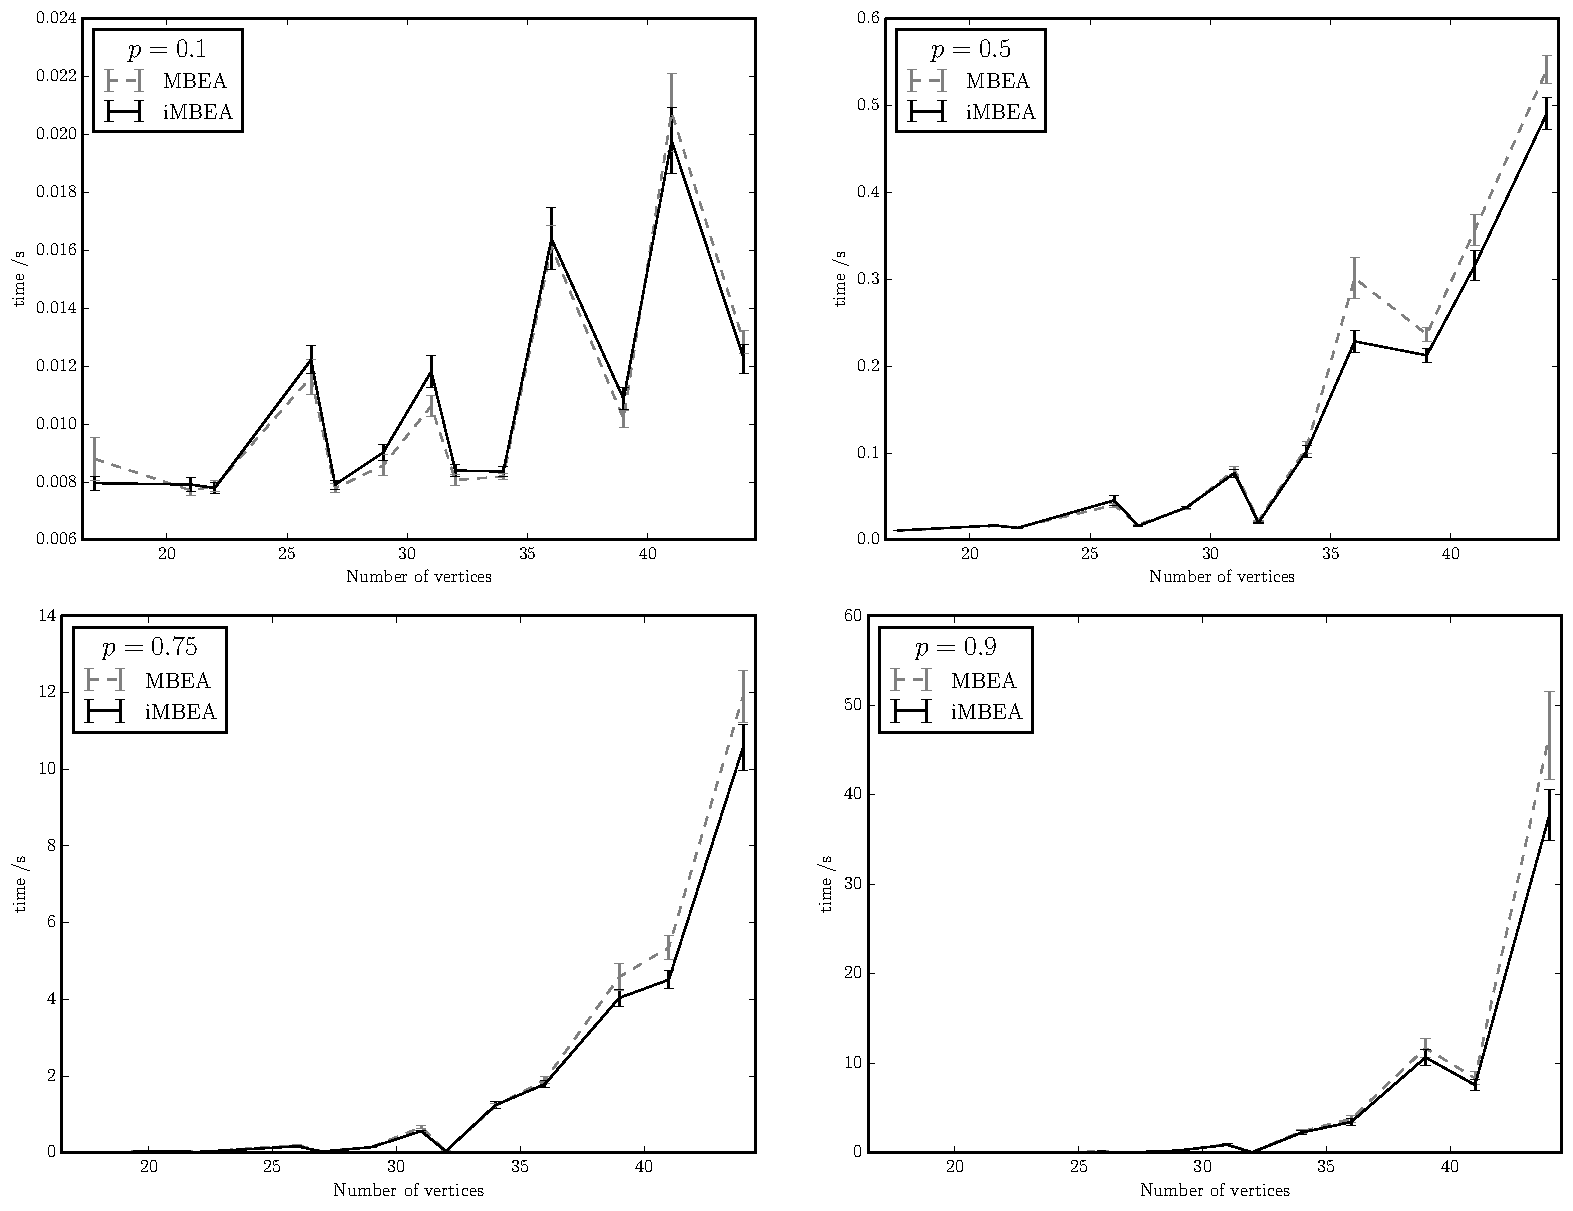
\includegraphics[width=0.95\textwidth]{plots}
    \caption{
    Results of experiment comparing implementations of MBEA and iMBEA.
    Note that in general, iMBEA runs faster, as one would expect from~\cite{Zhang2014}.
    Also note that as $p$ increases, i.e. the graphs get denser, the overall runtime increases.
    Error bars are standard error on the mean.
    }
    \label{fig:plots}
\end{figure}
\par
Observe that in general, iMBEA is faster than MBEA as expected.
An exception to this is in the $p=0.1$ where the graphs are more sparse.
iMBEA comes in to its own with the more dense graphs.
Also note that for dense graphs (with $p$ close to $1$) that the runtime starts approaching a minute for graphs on 45 vertices.

\section{Conclusions}
\subsection{Scalability}
\subsection{Design Improvements}
